% !TEX options=--shell-escape
\documentclass[10pt,titlepage]{scrartcl}

\usepackage[portuguese]{babel}
\selectlanguage{portuguese} 
\usepackage{pgfplots}
\usepackage{graphicx}
\usepackage{multirow}
\usepackage{makecell}
\usepackage{adjustbox}
\usepackage{url}
\usepackage[backend=biber, style=apa6]{biblatex}
\usepackage{textcomp}
\usepackage[bookmarksopen=true]{hyperref}
\usepackage{tikz}
\usepackage{xcolor}
\usepackage{geometry}
\usepackage{fancyhdr}
\usepackage[usestackEOL]{stackengine}
\usepackage{ragged2e}
\usepackage{todonotes}
\addbibresource{refs.bib}
\usepackage[acronym]{glossaries}
\makeglossaries

% FOOTER
\pagestyle{fancy}
\fancyhf{}
\renewcommand{\footrulewidth}{0pt}    
\renewcommand{\headrulewidth}{0pt}
\rfoot{\thepage}

\fancypagestyle{default_style}{
    \fancyhf{}
    \renewcommand{\footrulewidth}{1pt}
    \renewcommand{\headrulewidth}{0pt}
    \lfoot{Nuno Costa}
    \rfoot{\thepage}
}

% FRONTMATTER/MAINMATTER
\makeatletter

\newcommand\frontmatter{%
    \cleardoublepage
  %\@mainmatterfalse
  \pagenumbering{roman}}

\newcommand\mainmatter{%
    \cleardoublepage
 % \@mainmattertrue
  \pagenumbering{arabic}}

\newcommand\backmatter{%
  \if@openright
    \cleardoublepage
  \else
    \clearpage
  \fi
 % \@mainmatterfalse
   }

\makeatother

\setcounter{tocdepth}{4}

\begin{document}
\frontmatter
\begin{titlepage}
    \begin{center}
        \begin{tikzpicture}[remember picture,overlay]
            \node[anchor=north west,inner sep=0pt] at (current page.north west){
\includegraphics[height=2.4cm]{ISEP.png}};
            \node[anchor=north east,inner sep=0pt] at (current page.north east){
\includegraphics[height=1.8cm]{dei.png}};
        \end{tikzpicture}
        \vspace*{6cm}
        
        \textbf{\huge Cultura Organizacional}

        Caso de Estudo - Agência Continental
                    
        \vspace{4cm}
        
        \begin{table}[ht]
            \begin{tabular}{lp{1cm}l}
                \textbf{Turma 3DK - Grupo XX}           &   & \textbf{Docente}            \\
                1181184 - Diogo Leite de Pinho Oliveira &   & Sónia Sousa Nouws          \\
                1171584 - Nuno Costa                    &   &                             \\
                1181163 - Nuno Bastos Lima              &   & \textbf{Unidade Curricular} \\
                                                        &   & CORGA                       
            \end{tabular}
        \end{table}
        \vspace*{\fill}
        Abril,2021
                    
    \end{center}
\end{titlepage}

\newpage

\setcounter{page}{1}

%!TEX root = main.tex

\section*{Resumo}
\addcontentsline{toc}{section}{Resumo}

O presente relatório apresenta a organização Agência Continental, uma análise da mesma e uma descrição do processo de obtenção de dados, tudo no âmbito da Unidade Curricular de CORGA (Comportamento organizacional).

Foram distribuídos inquéritos, com base no modelo OCAI aos colaboradores da organização de modo a obter dados relativos à opinião destes sobre a cultura organizacional em que se encontram inseridos.

Após uma análise aos inquéritos, verificamos que, na sua maioria, os funcionários têm uma opinião positiva sobre a cultura organizacional da empresa. No entanto, existem sempre pontos fracos (ou menos positivos), que são também demonstrados na análise dos dados obtidos.

O processo de desenvolvimento deste trabalho foi uma experiência positiva na vertente profissional dos membros do grupo, na medida que nos permitiu adquirir uma nova visão no que toca à recolha e análise de dados num ambiente empresarial, para além da verificação das implicações da cultura organizacional no bem estar dos colaboradores e, subsequentemente, no sucesso da organização.

\subsection*{Palavras-chave:} 

Organização, Cultura Organizacional, Inquéritos, Análise de resultados, OCAI

\newpage
\tableofcontents

\newpage
%acronimos
\printglossary[type=\acronymtype]
\addcontentsline{toc}{section}{Lista de Acrónimos}

\newacronym{cvf}{CVF}{Competing Values Framework}

\newpage
%figuras
\listoffigures
\addcontentsline{toc}{section}{Lista de Figuras}

\newpage
%tabelas
\listoftables
\addcontentsline{toc}{section}{Lista de Tabelas}

\newpage

\mainmatter

%!TEX root = main.tex

\section{Introdução}

Este relatório, executado no âmbito da unidade curricular de Comportamento Organizacional da Licenciatura de Engenharia Informática do Instituto Superior de Engenharia do Porto, vai se incidir na análise da empresa Agência Continental Lda à luz dos conhecimentos e competências desenvolvidas no âmbito da unidade curricular.

\subsection{Objetivos}

Os objetivos deste trabalho são fazer uma descrição da organização concisa e fundamentada, através dos inquéritos distribuídos (e a sua respetiva análise), à luz dos fundamentos teóricos obtidos no curso da unidade curricular.

\subsection{A Empresa}
A empresa selecionada para análise foi a Agência Continental Lda. Esta disponibiliza serviços de contabilidade, aconselhamento de gestão, planeamento, preparação e \textit{outsourcing} para empresas. Tem também, dentro da sua estrutura empresarial, mediação de seguros (através da entidade Zeferino Barbosa - Mediação de Seguros, Lda.) e serviços de arquitetura (através da entidade Arquipaços - Gabinete de Projetos e Licenciamentos Industriais, Lda.) \parencite{agenciacontinental}.

A Agência Continental Lda. encontra-se sediada em Paços de Ferreira, com filiais em Raimonda, Penamaior e Paços de Ferreira.

A empresa emprega 80 funcionários em todas as suas sucursais.

\subsection{O Estudo}

Para analisar a cultura organizacional da empresa, foi distribuído um questionário a uma pequena amostra da força de trabalho da empresa.

Apesar de não termos feito uma análise completa, assumimos que foi obtida um amostra suficiente para uma análise complementar ao enquadramento teórico feito.

\subsection{O Relatório}

O desenvolvimento (e subsequente estrutura) deste relatório foi feito em 5 partes:

\begin{enumerate}
	\item Introdução
	\item Revisão da Literatura
	\item Caso Prático
	\item Conclusão
\end{enumerate}

Cada uma destas secções tem um pequeno prefácio.

%!TEX root = main.tex

\section{Revisão da Literatura}

A revisão de literatura consiste na apresentação, síntese e avaliação crítica da dita literatura, de modo a sustentar, de um ponto de vista teórico, a investigação efetuada.

É importante de referir que a cultura organizacional de uma empresa influência a própria organização. Deste modo, a cultura pode ser definida como um conjunto de ideias adquiridas ao longo do tempo que distinguem membros de diferentes grupos e a sua forma de reagir a diferentes situações \parencite{Schein_1990,Ravasi_Schultz_2006}.

As cultura organizacionais podem ser classificadas, subdivididas e comparadas através de vários modelos e teorias avançadas pela comunidade académica. Neste relatório e, no processo de análise da empresa em questão, vamos enquadrar a cultura da mesma em dois modelos: o modelo de Cameron \& Quinn e o modelo de Hofstede.

\subsection{Modelo de Cameron \& Quinn}

O modelo de Cameron \& Quinn \parencite{Cameron_Quinn_2011} define quatro tipos de culturas organizacionais, baseados na \acrfull{cvf} (inicialmente desenvolvido por professores na Universidade de Michigan \parencite{10.2307/3380029}). Estes quatro tipos de culturas podem ser representados num sistema de duas dimensões.

\begin{figure}[h]
\centering
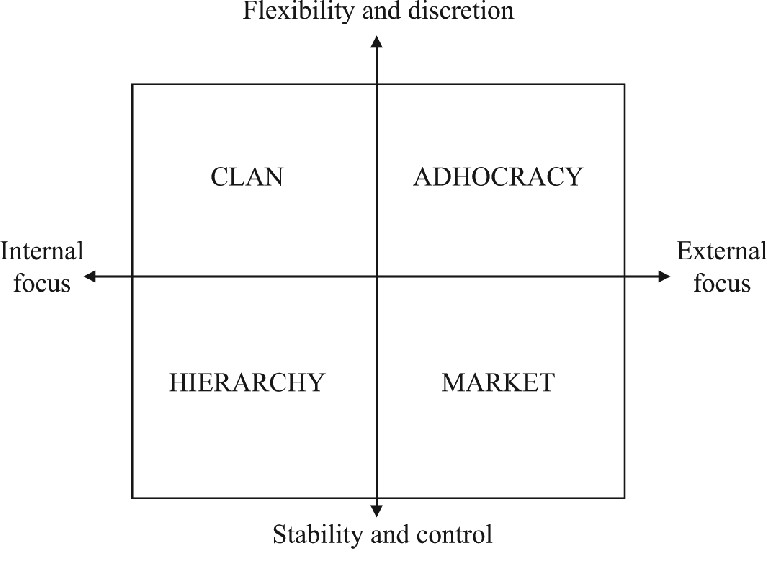
\includegraphics[width=0.5\textwidth]{cvf}
\caption{Modelo de Cameron \& Quinn}
\end{figure}

Estas dimensões definem uma dicotomia entre duas características de uma organização. Assim, a dimensão da flexibilidade/estabilidade impõe uma divisão entre organizações mais flexíveis e adaptáveis e, em contrapartida, organizações mais estáveis e controladoras. A dimensão de foco define uma dicotomia entre um foco de uma organização em processos internos ou em processos externos \parencite{diagnosing}.

Com estas divisões feitas, podemos definir os 4 tipos de culturas organizacionais:

\begin{itemize}
	\item \textit{Clan}
	\item \textit{Adhocracy}
	\item \textit{Hierarchy}
	\item \textit{Market}
\end{itemize}

\subsubsection{\textit{Clan}}

Esta cultura é definida por ter um foco interno e flexibilidade na manutenção da organização. Direciona-se para as pessoas afetas à organização. Esta tipologia é identificada, de forma geral, em organizações familiares.


\subsubsection{\textit{Adhocracy}}

Esta tipologia define uma cultura flexível e focada no mercado. Dá especial importância à inovação e empreendedorismo. Este tipo de organização é encontrado em mercados em rápido crescimento e com uma baixa aversão a risco.

\subsubsection{\textit{Hierarchy}}

Esta tipologia define uma cultura estável, controlada e com um foco interno. Enfatiza a eficiência e controlo dos processos organizacionais e a eliminação de erros. Este tipo de organização representa em grande parte organizações burocráticas com estruturas rígidas e bem-definidas.

\subsubsection{\textit{Market}}

Esta tipologia define uma cultura estável, controlado e com um foco no mercado. Assim, a organização está direcionada para a competição, em atingir objetivos. Esta tipologia adequa-se a empresas de marketing e vendas, por exemplo.

\subsection{Modelo de Hofstede}

No final do século XX, Geert Hofstede realizou um estudo em larga escala sobre as diferenças nos valores nacionais nas várias subsidiárias da empresa multinacional \acrfull{ibm}. Este estudo permitiu a Hofstede fazer comparações entre nações e realçar valores culturais que podem ser encontrados nos ambientes organizacionais. Hofstede posteriormente publicou um livro com os resultados desta pesquisa  \parencite{Hofstede_1981}.
 
Desse estudo resultou uma teoria chamada “A Teoria das Dimensões Culturais”. Esta permite examinar a forma como os valores culturais afetam o comportamento e as ações de pessoas de uma determinada cultura. A teoria divide-se em seis dimensões culturais: distância hierárquica, individualismo/coletivismo, aversão/incerteza, masculinidade/feminilidade, orientação em longo prazo e complacência/repressão.

\subsubsection{Distância hierárquica}

Aqui, o poder é distribuído de forma desigual, pois há uma necessidade de distinguir os superiores hierárquicos dos restantes. Estes últimos devem aceitar esta condição e esperar uma distribuição desigual do poder.

Neste conceito, a mudança acontece através de revoluções devido ao facto dos superiores hierárquicos terem privilégios.

\subsubsection{Individualismo vs Coletivismo}

O individualismo implica uma sociedade em que as decisões são tomadas de forma independente, em benefício próprio e com preocupações apontadas a si mesmo ou à família mais próxima.

Contrariamente, o coletivismo foca mais na relação dentro da sociedade do que nas tarefas individuais. Outro objetivo é  também manter a harmonia nos membros do grupo.

\subsubsection{Masculinidade vs Feminilidade}

Este fator tem como objetivo medir os graus dos valores associados ao sexo masculino e feminino.
Por um lado, sociedades onde a masculinidade prevalece, as pessoas são guiadas mais pelos resultados e ambição. Nestes casos, os conflitos são resolvidos de modo a vencerem os mais fortes.

Por outro lado, numa sociedade onde a feminilidade prevalece, a qualidade de vida é o foco principal juntamente com a harmonia interpessoal. Nestas situações, a sociedade tende a construir boas relações e sentir mais compaixão pelos menos afortunados.

\subsubsection{Evitamento da incerteza}

Este parâmetro representa a sensação de insegurança, desconforto e até medo que os colaboradores adotem perante o desconhecido, seja ele situações de risco, incertezas, imprevistos, etc. Este parâmetro varia de cultura para cultura e naquelas em que o índice de aversão à incerteza é mais elevado, as pessoas tendem a adotar um comportamento mais seguro de modo a evitar estas situações de risco e se sentirem melhor.

Os espaços culturais onde se identifica este comportamento e onde fugir à rotina significa maior ansiedade e stress são: Japão, Rússia, Grécia. Já em culturas onde o índice de aversão à incerteza é mais baixo, a sociedade adapta-se mais facilmente a situações de risco e incerteza sendo mais flexíveis dependendo das circunstâncias.

\subsubsection{\textit{Long-term vs short-term orientation}}

Em culturas onde o pensamento a longo prazo está constantemente presente, este é uma forma de incentivar a população a gerir melhor a sua economia, tendo a noção que os resultados poderão vir a aparecer lentamente, demonstrando assim serem pessoas pacientes, esforçadas e perseverantes. Com isto, estas apresentam estar dispostas a gerir os seus objetivos, sacrificando objetivos presentes por objetivos futuros mais recompensantes, ou seja frutos dos seus investimentos. 

Culturas que pensam a curto prazo são mais conservadoras e demonstram ser mais tradicionais. Defendem e incentivam o consumo, gastos e objetivos de curto prazo. Nestas sociedades, a “label” social imposta pelas pessoas envolventes é muito importante. Não demonstram grande importância com o que o futuro representa mas sim grande importância em viver o presente. Pode-se concluir que há uma grande pressão social relacionado com o estilo de vida de cada um e a imagem pública de cada um.

\subsubsection{Indulgência vs Restrição}

A predominância da indulgência numa população demonstra que a sua cultura valoriza o bem-estar e conexão humana. Procuram a satisfação de necessidades básicas e desejos. Não são pessoas materialistas, mas sim pessoas muito ligadas sentimentalmente entre si, o que leva a serem pessoas mais sociáveis, extrovertidas e amigáveis. Sendo assim estas pessoas mais facilmente conseguem apresentar empatia e perdoar o próximo.

Já em culturas onde predomina a restrição, a disciplina moral é muito relevante e importante. Existem normas sociais restritivas onde as pessoas sentem que os seus sentimentos são oprimidos prejudicando o seu bem-estar, tornando-as mais pessimistas, deprimidas e facilmente injustiçadas. São sociedades materialistas e que sobrevalorizam o seu status aos olhos da sociedade.

%!TEX root = main.tex

\section{Caso Prático}

Nesta secção é apresentada a empresa em análise e as suas dimensões relevantes. É também apresentado os resultados da pesquisa efetuada, análise dos mesmos e comparação com o enquadramento teórico referido na secção anterior.

\subsection{A Empresa}

A empresa selecionada para análise foi a Agência Continental Lda. Esta disponibiliza serviços de contabilidade, aconselhamento de gestão, planeamento, preparação e \textit{outsourcing} para empresas. Tem também, dentro da sua estrutura empresarial, mediação de seguros (através da entidade Zeferino Barbosa - Mediação de Seguros, Lda.) e serviços de arquitetura (através da entidade Arquipaços - Gabinete de Projetos e Licenciamentos Industriais, Lda.) \parencite{agenciacontinental}.

A Agência Continental Lda. encontra-se sediada em Paços de Ferreira, com filiais em Raimonda, Penamaior e Paços de Ferreira.

A empresa emprega 80 funcionários em todas as suas sucursais.

\subsubsection{História}

A Agência Continental Lda. foi fundada no final da década de 60 \parencite{agenciacontinental}. Fundada no início da explosão da indústria (com um ênfase no mobiliário) em Paços de Ferreira, serviu de trampolim para vários industriais que aventuraram-se no mercado. Começou com apenas 4 pessoas, crescendo continuamente até aos 80 colaborados que hoje se associam à mesma.

Mudou de instalações por três vezes, sempre com o intuito de acomodar mais colaboradores. Para além das instalações principais situadas no centro da cidade de Paços de Ferreira, fundou a também a primeira filial em 1999, na freguesia de Figueiró, de modo a melhor servir os clientes lá localizados. Abriu uma segunda filial em 2010, na freguesia de Penamaior, com os mesmos objetivos. Mais recentemente expandiu os serviços disponibilizados, com a abertura de uma loja de seguros, também no centro de Paços de Ferreira.

Com um desenvolvimento empresarial ativo, angariou durante a sua atividade um carteira de clientes elevada, sendo uma das maiores empresas a nível nacional na área.

\subsubsection{Missão e Visão}

A missão da Agência Continental Lda. é apoiar as decisões de gestão empresarial, através de soluções que maximizem a eficácia e eficiência da gestão dos recursos, contribuir para a afirmação competitiva e sustentada das organizações através da transferência de conhecimento, experiências e valores, promovendo o desenvolvimento de competências.

A empresa em análise tem como visão ser vista pelos seus clientes e mercados em que opera como uma empresa de excelência em serviços para empresas e indivíduos, ocupando um lugar importante na sua hierarquia\parencite{agenciacontinental}.

\subsubsection{Valores}

A empresa tem como valores Integridade, Qualidade e Melhoria Contínua \parencite{agenciacontinental}.

\paragraph{Integridade} No sentido de facultar aos seus clientes uma resposta honesta e correta a todas as questões que possam ter, para além de atingir os objetivos fixados, dentro do tempo previsto.

\paragraph{Qualidade} Na forma em que nivela todas as ações por um patamar de elevada qualidade e tem como objetivo último, superar as expectativas que os clientes têm relativamente à mesma.

\paragraph{Melhoria Contínua} No sentido de estimular o trabalho em equipa, apelando a valores como a colaboração, proatividade e dinamismo, para além de fazer um constante investimento na qualificação dos seus colaboradores.

\subsubsection{Logótipo e Slogan}

O logótipo da Agência Continental Lda. mantém-se inalterado desde a sua concepção, sendo apenas atualizado com cores (visto o logótipo original ser a preto e branco).

\begin{figure}[h]
\centering

\includegraphics[width=0.5\textwidth]{ag_continental}
\caption{Logótipo da Agência Continental}
\end{figure}

A empresa tem como slogan ``Simplificamos o seu negócio'', aludindo aos serviços disponibilizados e ao fator de simplificação dos deveres fiscais e legais de uma empresa ao utilizar os serviços disponibilizados pela Agência Continental Lda..

\subsection{Análise}


\subsubsection{Interna}


\subsubsection{Externa}



\input{conclusao}

\newpage

\printbibliography

\newpage

\end{document}